\chapter{Joshua 13}

\begin{figure}
  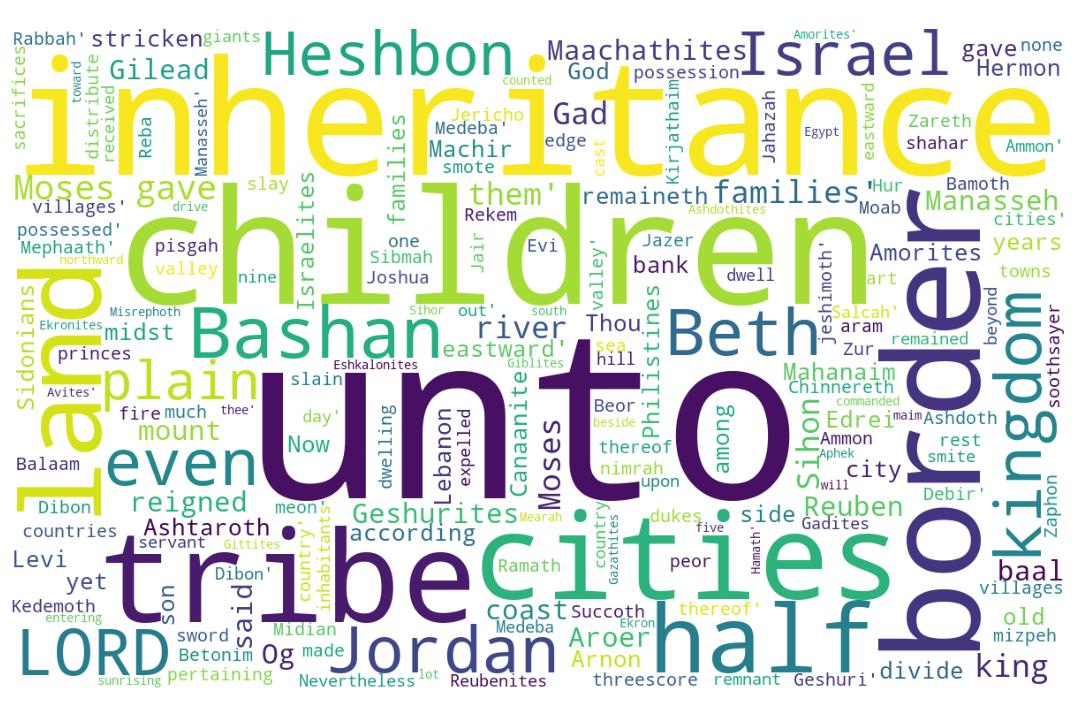
\includegraphics[width=\linewidth]{06OT-Joshua/Joshua13-WordCloud.jpg}
  \caption{Joshua 13 Word Cloud}
  \label{fig:Joshua 13 Word Cloud}
\end{figure}

\marginpar{\scriptsize \centering \fcolorbox{bone}{lime}{\textbf{FINISH THE JOB}}\\ (Joshua 13) \begin{compactenum}[I.][8]
	\item A \textbf{Duty} (to conquer and possess) \index[scripture]{Joshua!Jsh 13:02}  (Jsh 13:2) 
	\item The \textbf{Driving Out} (by God) \index[scripture]{Joshua!Jsh 13:06}  (Jsh 13:6) 
	\item The original \textbf{Divide} and Conquer  \index[scripture]{Joshua!Jsh 13:07}  (Jsh 13:7) 
	\item The \textbf{Distribution} to Rueben \index[scripture]{Joshua!Jsh 13:15--23}  (Jsh 13:15--23) 
	\item The \textbf{Dukes} \index[scripture]{Joshua!Jsh 13:21}  (Jsh 13:21) 
	\item The \textbf{Dwellingplaces} \index[scripture]{Joshua!Jsh 13:21}  (Jsh 13:21) 
	\item A \textbf{Distinct} Place \index[scripture]{Joshua!Jsh 13:33}  (Jsh 13:33) 
\end{compactenum}}




\footnote{\textcolor[rgb]{0.00,0.25,0.00}{\hyperlink{TOC}{Return to end of Table of Contents.}}}\footnote{\href{https://audiobible.com/bible/joshua_13.html}{\textcolor[cmyk]{0.99998,1,0,0}{Joshua 13 Audio}}}\textcolor[cmyk]{0.99998,1,0,0}{Now Joshua was old \emph{and} stricken in years; and the LORD said unto him, Thou art old \emph{and} stricken in years, and there remaineth yet very much land to be possessed.}
[2] \textcolor[cmyk]{0.99998,1,0,0}{This \emph{is} the land that yet remaineth: all the borders of the Philistines, and all Geshuri,}
[3] \textcolor[cmyk]{0.99998,1,0,0}{From Sihor, which \emph{is} before Egypt, even unto the borders of Ekron northward, \emph{which} is counted to the Canaanite: five lords of the Philistines; the Gazathites, and the Ashdothites, the Eshkalonites, the Gittites, and the Ekronites; also the Avites:}
[4] \textcolor[cmyk]{0.99998,1,0,0}{From the south, all the land of the Canaanites, and Mearah that \emph{is} beside the Sidonians, unto Aphek, to the borders of the Amorites:}
[5] \textcolor[cmyk]{0.99998,1,0,0}{And the land of the Giblites, and all Lebanon, toward the sunrising, from Baal-gad under mount Hermon unto the entering into Hamath.}
[6] \textcolor[cmyk]{0.99998,1,0,0}{All the inhabitants of the hill country from Lebanon unto Misrephoth-maim, \emph{and} all the Sidonians, them will I drive out from before  \fcolorbox{bone}{bone}{the children of} Israel: only divide thou it by lot unto the Israelites for an inheritance, as I have commanded thee.}
[7] \textcolor[cmyk]{0.99998,1,0,0}{Now therefore divide this land for an inheritance unto the nine tribes, and the half tribe of Manasseh,}
[8] \textcolor[cmyk]{0.99998,1,0,0}{With whom the Reubenites and the Gadites have received  \fcolorbox{bone}{bone}{their} inheritance, which Moses gave them, beyond Jordan eastward, \emph{even} as Moses the servant of the LORD gave them;}
[9] \textcolor[cmyk]{0.99998,1,0,0}{From Aroer, that \emph{is} upon the bank of the river Arnon, and the city that \emph{is} in the midst of the river, and all the plain of Medeba unto Dibon;}
[10] \textcolor[cmyk]{0.99998,1,0,0}{And all the cities of Sihon king of the Amorites, which reigned in Heshbon, unto the border of  \fcolorbox{bone}{bone}{the children of} Ammon;}
[11] \textcolor[cmyk]{0.99998,1,0,0}{And Gilead, and the border of the Geshurites and Maachathites, and all mount Hermon, and all Bashan unto Salcah;}
[12] \textcolor[cmyk]{0.99998,1,0,0}{All the kingdom of Og in Bashan, which reigned in Ashtaroth and in Edrei, who remained of the remnant of the giants: for these did Moses smite, and cast them out.}
[13] \textcolor[cmyk]{0.99998,1,0,0}{Nevertheless  \fcolorbox{bone}{bone}{the children of} Israel expelled not the Geshurites, nor the Maachathites: but the Geshurites and the Maachathites dwell among the Israelites until this day.}
[14] \textcolor[cmyk]{0.99998,1,0,0}{Only unto the tribe of Levi he gave none inheritance; the sacrifices of the LORD God of Israel made by fire \emph{are}  \fcolorbox{bone}{bone}{their} inheritance, as he said unto them.}\\
\\
\P  \textcolor[cmyk]{0.99998,1,0,0}{And Moses gave unto the tribe of  \fcolorbox{bone}{bone}{the children of} Reuben \emph{inheritance} according to  \fcolorbox{bone}{bone}{their} families.}
[16] \textcolor[cmyk]{0.99998,1,0,0}{And  \fcolorbox{bone}{bone}{their} coast was from Aroer, that \emph{is} on the bank of the river Arnon, and the city that \emph{is} in the midst of the river, and all the plain by Medeba;}
[17] \textcolor[cmyk]{0.99998,1,0,0}{Heshbon, and all her cities that \emph{are} in the plain; Dibon, and Bamoth-baal, and Beth-baal-meon,}
[18] \textcolor[cmyk]{0.99998,1,0,0}{And Jahazah, and Kedemoth, and Mephaath,}
[19] \textcolor[cmyk]{0.99998,1,0,0}{And Kirjathaim, and Sibmah, and \fcolorbox{bone}{MYGOLD}{Zareth-shahar} in the mount of the valley,}
[20] \textcolor[cmyk]{0.99998,1,0,0}{And Beth-peor, and Ashdoth-pisgah, and Beth-jeshimoth,}
[21] \textcolor[cmyk]{0.99998,1,0,0}{And all the cities of the plain, and all the kingdom of Sihon king of the Amorites, which reigned in Heshbon, whom Moses smote with the princes of Midian, Evi, and Rekem, and Zur, and Hur, and Reba, \emph{which} \emph{were} dukes of Sihon, dwelling in the country.}\\
\\
\P  \textcolor[cmyk]{0.99998,1,0,0}{Balaam also the son of Beor, the soothsayer, did  \fcolorbox{bone}{bone}{the children of} Israel slay with the sword among them that were slain by them.}
[23] \textcolor[cmyk]{0.99998,1,0,0}{And the border of  \fcolorbox{bone}{bone}{the children of} Reuben was Jordan, and the border \emph{thereof}. This \emph{was} the inheritance of  \fcolorbox{bone}{bone}{the children} \fcolorbox{bone}{bone}{of} Reuben after  \fcolorbox{bone}{bone}{their} families, the cities and the villages thereof.}
[24] \textcolor[cmyk]{0.99998,1,0,0}{And Moses gave \emph{inheritance} unto the tribe of Gad, \emph{even} unto  \fcolorbox{bone}{bone}{the children of} Gad according to  \fcolorbox{bone}{bone}{their} families.}
[25] \textcolor[cmyk]{0.99998,1,0,0}{And  \fcolorbox{bone}{bone}{their} coast was Jazer, and all the cities of Gilead, and half the land of  \fcolorbox{bone}{bone}{the children of} Ammon, unto Aroer that \emph{is} before Rabbah;}\
[26] \textcolor[cmyk]{0.99998,1,0,0}{And from Heshbon unto \fcolorbox{bone}{MYGOLD}{Ramath-mizpeh}, and Betonim; and from Mahanaim unto the border of Debir;}
[27] \textcolor[cmyk]{0.99998,1,0,0}{And in the valley, Beth-aram, and Beth-nimrah, and Succoth, and Zaphon, the rest of the kingdom of Sihon king of Heshbon, Jordan and \emph{his} border, \emph{even} unto the edge of the sea of Chinnereth on the other side Jordan eastward.}
[28] \textcolor[cmyk]{0.99998,1,0,0}{This \emph{is} the inheritance of  \fcolorbox{bone}{bone}{the children of} Gad after  \fcolorbox{bone}{bone}{their} families, the cities, and  \fcolorbox{bone}{bone}{their} villages.}\\
\\
\P \textcolor[cmyk]{0.99998,1,0,0}{And Moses gave \emph{inheritance} unto the half tribe of Manasseh: and \emph{this} was \emph{the} \emph{possession} of the half tribe of  \fcolorbox{bone}{bone}{the children of} Manasseh by  \fcolorbox{bone}{bone}{their} families.}
[30] \textcolor[cmyk]{0.99998,1,0,0}{And  \fcolorbox{bone}{bone}{their} coast was from Mahanaim, all Bashan, all the kingdom of Og king of Bashan, and all the towns of Jair, which \emph{are} in Bashan, threescore cities:}
[31] \textcolor[cmyk]{0.99998,1,0,0}{And half Gilead, and Ashtaroth, and Edrei, cities of the kingdom of Og in Bashan, \emph{were} \emph{pertaining} unto  \fcolorbox{bone}{bone}{the children of} Machir the son of Manasseh, \emph{even} to the one half of  \fcolorbox{bone}{bone}{the children of} Machir by  \fcolorbox{bone}{bone}{their} families.}
[32] \textcolor[cmyk]{0.99998,1,0,0}{These \emph{are} \emph{the} \emph{countries} which Moses did distribute for inheritance in the plains of Moab, on the other side Jordan, by Jericho, eastward.}
[33] \textcolor[cmyk]{0.99998,1,0,0}{But unto the tribe of Levi Moses gave not \emph{any} inheritance: the LORD God of Israel \emph{was}  \fcolorbox{bone}{bone}{their} inheritance, as he said unto them.}
